\documentclass[font=plain]{abnt}
\usepackage[utf8]{inputenc}
\usepackage[brazil]{babel}
\usepackage[title, abnt-etal-cite=3]{abntcite}
\usepackage{graphicx}
\usepackage{graphicx,color} 
\usepackage{placeins} % para posicionamento das imagens
\usepackage{paralist}
\usepackage{subfloat} 
\usepackage{subfig} 
\usepackage{multirow}
\usepackage{lscape}

\usepackage{amsmath,amsfonts}   % \mathbb, para fontes matematicas
\usepackage{amssymb,amsthm}  
\instituicao{UNEB - Universidade do Estado da Bahia 
             \par Departamento de Ciências Exatas e da Terra}
\titulo{Planejamento adaptativo de trajetórias em tempo real para navegação de robôs humanóides no contexto de jogo de futebol em ambiente simulado 3D}
\autor{Alan dos Santos Soares}
\orientador{Diego Gervasio Frías Suárez}

\comentario{Análise de estabilidade, Navega\c{c}\~ao, Locomoção Bípede, Simula\c{c}\~ao 3D}
\local{Rua Silveira Martins, 2555, Cabula, Salvador-BA}
%esta data deve ficar estática após entrega final
\data{\today}

\begin{document}
\capa
\folhaderosto

%%%%%%%%%%% Folha de Aprovação
\begin{folhadeaprovacao}
\begin{center}
\large
\textbf{Folha de Aprovação}
\end{center}

\setlength{\ABNTsignthickness}{0.4pt}
\setlength{\ABNTsignskip}{2cm}
\hspace*{1cm}
 \assinatura{Prof. PhD. Diego Gervasio Frías Suárez\\Orientador}
\end{folhadeaprovacao}

\chapter{Introdução}

A organização internacional Robocup foi formada com o intuito de promover pesquisas nas áreas de robótica e inteligência artificial
através da construção de plataformas estimulantes que estão fundamentadas em problemas do mundo real.

Dentre as várias plataformas da Robocup encontra-se a simulação 3D, sub-liga da \textit{robocup soccer}, e a primeira dentre as simuladas 
a representar um robô humanóide em sua competição. O principal objetivo dessa categoria é o desenvolvimento do controle de baixo nível de
robôs humanóides e a criação de comportamentos básicos e eficientes como levantar, correr, entre outros.\cite{SimulationLeague}

Este projeto tem como objetivo desenvolver um modelo de busca de trajetórias eficientes para os robôs humanóides no contexto do jogo 
de futebol simulado 3D. 
%e  para o desafio proposto de vencer o time de humanos campeão da última Copa do Mundo da FIFA, utilizando
%as regras da FIFA \cite{RobocupHistory}.

\chapter{Justificativa}
%Faça a justificativa desse tema. Por quais motivos essa pesquisa é relevante e importante? Apresente argumentos que justificam a importância da pesquisa no âmbito do seu campo de conhecimento e a relevância social do estudo (motivos e relevância da escolha do tema, levando em conta formação pessoal e pertinência/ contribuição acadêmica).
Um dos principais desafios no campo da robótica, é a forma como os agentes humanóides realizam a trajetória para chegar a 
um determinado objetivo. No ambiente em que o agente está atuando podem existir diversos obstáculos que podem comprometer 
a sua locomoção no ambiente. Fazer com que o agente se mova de uma posição e orientação para uma outra posição e orientação
desejada encontrando o menor caminho e evitando colidir com os objetos que dificultam a sua locomoção é fundamental para que
o agente consiga chegar no tempo mínimo no local desejado.

Animação de personagens, design, fabricação farmacêutica, exploração e mapeamento de ambientes desconhecidos e de controle de
alto nível de veículos autônomos são apenas alguns dos problemas impactados pela área de planejamento de trajetória.

Existem diversos algoritmos que tratam da navegação de agentes humanóides, sendo que um dos primeiros é descrito no livro de
Inteligência Artificial de Russell e Norvig, o algorítmo A* \cite{brussel}. Ele busca o caminho em um grafo de
um vértice inicial até um vértice final, é a combinação de aproximações heurísticas como do algoritmo Best-first Search e da
formalidade do Algoritmo de Dijkstra (DIJKSTRA, 1959).

O estudo e desenvolvimento do projeto na área de robôs humanóides simulados jogadores de futebol, atende à necessidade estratégica
de continuar criando competências e desenvolvendo know-how próprio no estado da Bahia e no país na área de robótica autônoma para
não sermos, em um futuro imediato meros consumidores de tecnologia desenvolvida em outros estados e outros países.

Além disso, o estudo tem como objetivo melhorar a performance dos agentes do time BahiaRT do ACSO(Nucleo de Arquitetura de 
Computadores e Sistemas Operacionais) da UNEB, mais especificamente no grupo 3D, que é o de agentes simulados 3D, que tem como objetivo
construir agentes totalmente autônomos e inteligentes e vencer a sub-liga 3D da Robocup.

\chapter{Objetivo}
%Defina o objetivo da pesquisa. No que a pesquisa contribuirá? Aqui, você poderá detalhar em objetivo geral e objetivos específicos, pois isso dependerá da extensão da sua pesquisa.
O objetivo do trabalho é propor e validar um modelo de planejamento de trajetórias mínimas de agentes humanóides no ambiente simulado 
3D no contexto de jogo de futebol de robôs.

\section{Objetivos Específicos}
\begin{enumerate}
%\item Definir a especificação PEAS do ambiente
\item Calcular a trajetória prevista de todos os obstáculos
\item Definir o critério de acurácia dos obstáculos % não to nem ai pra você ! ...tipo isso
\item Definir o critério de descarte de trajetória prevista
\item Calcular a configuração objetivo final
\item Calcular a trajetória mínima a ser seguida até o objetivo
\end{enumerate}


%Fundamentacao Teorica
%Inicio falando sobre a importancia
%Planejamento de trajetória
%Algorítmo R*
%Geração de marcha
%Abordagem Híbrida
%Footstep Planning


\chapter{Fundamentação Teórica}

\section{Planejamento de trajet\'oria}
O objetivo principal da zona de planejamento de trajetória é a construção de algoritmos para automatizar o movimento de robôs, 
peças e outros ambientes que utilizam objetos geométricos arbitrários. A tarefa básica é mover um robô em seu ambiente de trabalho 
a partir de uma posição e orientação para outra posição e orientação desejada, sem o robô bater em obstáculos. O planejamento de 
movimento tem aplicações tanto dentro como fora da área de robótica.

O problema de navegação mais básico é mover um robô modelado como um ponto no espaço através de um ambiente bidimensional com vários
itens proibidos (ou obstáculo ), as regiões que o robô não pode entrar. O modelo é cinemático, o que significa que a única limitação
é que o robô tem de se mover ao longo de uma trajetória contínua.

O robô é modelado como um ponto no espaço de configuração, em vez de o espaço de trabalho. Uma configuração é uma especificação
do local (localização e orientação) do robô em relação ao meio ambiente e o espaço de configuração é o conjunto de todas as configurações
possíveis \cite{achoset}.

Realizar o planejamento apresenta um maior nível de complexidade quando o robô tem muitos graus de liberdade e orientação. Um robô 
guia pode passar por um espaço com uma certa posição e orientação, e atinge um obstáculo se fosse em uma orientação diferente. Isso 
aumenta a complexidade dos algoritmos para planejamento de trajetória.

O exemplo clássico de planejamento de trajetória é o problema do mecanismo de enfileiramento \cite{bsharir}: 
mover um piano através de uma casa de piano para não colidir com outros objetos na casa (ou a própria casa). Apenas considerou a 
geometria dos objetos e não as forças que atuam sobre o piano, como a gravidade .

Estendendo a analogia, o piano é suposto ter motores infinitamente fortes e infinitamente pequeno. Portanto, o problema do motor 
de piano só lida a circulação de uma forma geométrica ao longo de um caminho que é contínuo no espaço através de uma atmosfera.

Finalmente, talvez o mais difícil de restrição está relacionada com a estética do movimento. Pode ser desejável, para os movimentos 
do robô, para imitar o movimento humano. Por estas razões, os métodos baseados em amostra, não parecem ser a solução para o planejamento
de movimento humanóide.
%Porque os métodos baseados em amostra não são a solução para o planejamento de movimento humanóide

\section{Algorítmo R*}

Pesquisas heurísticas ótimas, como uma pesquisa A* são amplamente usadas para planejamento, mas raramente podem escalar para grandes problemas complexos. 
As versões sub-ótimas de buscas heurísticas, tais como pesquisa A*, muitas vezes podem ser escaladas para problemas de planejamento maiores, trocando 
a qualidade da solução para a eficiência. Elas fazem isso contando mais com a capacidade da função heurística para orientá-los bem para o gol. Para
problemas complexos de planejamento, no entanto, a função heurística muitas vezes pode orientar a busca em um grande mínimo local e fazer a busca 
examinar a maioria dos estados no mínimo local antes de prosseguir.

A busca heurística, denominada Busca R*\cite{plikhachev}, depende muito menos da qualidade da função heurística. A busca evita mínimos locais, resolvendo
o problema de planejamento de toda uma série de pesquisas de curto alcance e fácil de resolver, cada um guiado pela função heurística para um objetivo
escolhido aleatoriamente. Além disso, muitas escalas R* são melhores em termos de memória, pois podem descartar uma pesquisa no espaço-estado após 
cada uma de suas pesquisas. O algoritmo possui garantias probabilísticas em sub-otimização da solução devolvido por R* e pode ser dimensionado para
grandes problemas complexos.

Em vez de executar uma única pesquisa focada no sentido de um estado meta, R* tenta executar uma série de buscas ponderada A* de curto alcance no sentido 
de escolher estados meta aleatoriamente e reconstruir uma solução dos caminhos produzido por essas pesquisas. A principal idéia por R* baseia-se que ao 
invés de executar cada uma de suas pesquisas de curto alcance até que encontre soluções, R* adia os que não encontram soluções facilmente e tenta construir
a solução global usando apenas os resultados das pesquisas que encontrar soluções facilmente. 

%Rever a traducao dessa parte, está estranho
Programações e reprogramações de pesquisas de curto alcance são formas de dar garantias probabilísticas na sub-otimização da solução global que encontra. 
O algoritmo também possui sub-otimização ao segurar com probabilidade igual a 1 se R* não realiza down-select randomizado, do que agendar pesquisas de curto 
alcance. O algoritmo pode encontrar soluções para esses problemas com muito mais frequência do que pesquisa ponderada A*, e pode minimizar o custo de
encontrar soluções muito melhores do que os algoritmos de planejamento de movimento ao acaso, desenvolvidos especificamente para domínios contínuos.

\section{Geração de marcha}
Devido à complexidade do problema de planejamento de trajetórias, os investigadores e engenheiros frequentemente concentram-se 
em gerar movimentos curtos, tais como um único passo, ou repetindo andamentos em um ambiente livre de obstáculos. Este problema 
de geração de marcha é a segunda dificuldade núcleo de planejamento de movimento para caminhar robôs.

Sistemas mecânicos do andar de um robô não são facilmente controladas. Um robô andando tem uma dinâmica de sistemas não-lineares. 
Este sistema de equações terá apenas uma pequena gama de trajetórias que mantêm robô caindo, uma exigência da estabilidade, e as 
entradas de controle para o sistema será limitado como os motores só podem exercer um torque de até algum valor máximo. Este modelo 
matemático é geralmente difícil de analisar e não pode mesmo ter, uma solução explícita de forma fechada. Mesmo ignorando a geometria 
do ambiente, métodos de geração de marcha devem levar em consideração as colisões entre os elos do robô (auto-colisões). Além disso, 
as dificuldades de modelagem adicionais entram em jogo. O contato entre o pé de apoio do robô  e o solo não é um conjunto perfeito. O 
pé de apoio pode escorregar em momentos em que ela não deve se mover, e o atrito pode fazer mover-se difícil um pé de apoio. Além 
disso, o modelo deve considerar a força de impacto aplicada ao pé nos primeiros contatos do robô no solo e as forças de fricção na articulação.

Este problema da geração de marcha não é simples. Um número de abordagens são comumente feitas. Uma abordagem é desenvolver uma marcha
e projetar um controlador para controlar um padrão de movimentos articulares. Andamentos são gerados manualmente em alguns casos, pela
intuição de um designer humano ou por meio de captura de movimento para imitar diretamente o movimento humano \cite{bchoi}. 

Embora estes métodos dependem muito de uma trajetória predefinida, uma segunda abordagem baseia-se fortemente no feedback para 
estabilizar o robô. Políticas de controle com base no ponto do momento zero  do robô \cite{pkajita} \cite{pnagasaka} são exemplos comuns 
desta metodologia. Ao olhar e controlar os indicadores de comportamento do sistema, tais como o centro de massa, centro de pressão, 
ou ponto de momento zero, os controles que são projetados produzem (tipicamente) gerações estaticamente estáveis.

Apesar de não serem obrigados a seguir uma trajetória específica, estes métodos de feedback, especialmente de ponto de momento zero,
são em grande parte de energia ineficiente. Os custos do transporte (COT) é uma medida da eficiência de conversão de um sistema 
mecânico de energia para locomoção. Essencialmente, é a quantidade de energia consumida dividido pelo peso e pela distância percorrida
\cite{bkuo}. Por exemplo, o Asimo , da Honda , que utiliza o controle ponto de momento zero, tem um COT de 3,2 , que é 
cerca de dez vezes o COT de um ser humano.

Uma fusão de ambos geração marcha e planejamento de trajetória é útil para o planejamento de movimento bípede. Ambos planejamento de 
trajetória e métodos de geração de marcha têm desvantagens. No entanto, quando combinados de uma forma coordenada, eles podem amplificar 
sucessos um do outro enquanto parcialmente atenuar as deficiências do outro.

\section{Abordagem H\'ibrida}
Levando em considera\c{c}\~ao que o planejamento de trajet\'oria e problemas de controle s\~ao conhecidos por serem dif\'iceis, 
tanto analiticamente e computacionalmente, algumas abordagens para a navega\c{c}\~ao de rob\^os human\'oides s\~ao baseadas em 
uma simplifica\c{c}\~ao do modelo de planejamento de movimento human\'oide.

Planejamento de trajetória para um robô humanóide em terreno plano pode ser considerado como uma busca por uma seqüência de movimentos
primitivos vi\'aveis ao inv\'es de uma busca de um espa\c {c}o de configura\c{c}\~ao dimensional elevado para uma trajetória \cite{bkuffner}. 
O algoritmo de busca pode, em muitos casos, encontrar rapidamente uma seqüência de movimentos para levar o robô para o seu destino. No entanto,
a pesquisa vai exigir exponencialmente mais cheques como o número de primitivas de movimento naquele caminho. Em ambientes com obstáculos, 
escadas, rampas e buracos , os movimentos de humanóides são constrangidos por mais do que apenas a colocação do robô no plano. Um grande 
conjunto de primitivas de movimento é necessário para atravessar esses ambientes. Um algoritmo de programação dinâmica, uma pesquisa * ou
para frente pode levar um tempo considerável para calcular uma seqüência de primitivas de movimento ou o problema pode tornar-se 
computacionalmente intratável. Algumas abordagens de planeamento hierárquicos têm sido aplicados para controlar o crescimento de complexidade 
e encontrar uma solução para este problema aproximado \cite{pchesnutt}.

\section{Planejamento de Passo}
O planejamento de passo eficiente para navegação humanóide através de ambientes desordenados ainda é um problema desafiador. Muitos obstáculos
criam mínimos locais no espaço de busca, forçando planejadores heurísticos, tais como o A* para expandir grandes áreas.

Abordagens populares de cálculo de passo eficiente para trajetórias dado um conjunto finito de ações com passo eficiente que são executáveis
pelo robô para fazer a busca de caminhos livres de colisão tratável. Um controlador de pé, em seguida, calcula a trajetória do angulo das juntas 
para caminhar nos passos planejados. A pesquisa no espaço de estados de passos fica realizada ou usando um método baseado no A* incluindo variantes dinâmicas 
\cite{phornung} \cite{pgarimort} ou métodos randomizados\cite{bperrin}. Enquanto o A* vai encontrar o caminho ideal para parametrizção de um 
determinado passo e discretização do estado, o seu desempenho depende fortemente da qualidade da função heurística que orienta a pesquisa, mais não 
tem quaisquer garantias sobre a qualidade da solução do caminho final. Além disso, muitas vezes eles dependem do alisamento do caminho 
final em um fase de pós-processamento.

Este método leva inerentemente a capacidade de robôs humanóides para passar por cima de obstáculos. Um conjunto discreto de
transições de passo, ilustrado na figura \ref{fig:footstep}, é utilizado em uma heurística de busca tais como A*\cite{bperrin}. Por este meio, estados 
constituem a posição e orientação $( x, y, \theta )$ do pé de apoio atual. O próximo estado pode ser alcançado através da aplicação da ação de 
um dos passos possíveis e mudando o pé de apoio.

\begin{figure}[h]

\centering

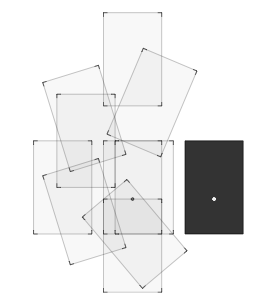
\includegraphics[scale=0.48]{figuras/footstep.png}

\caption{Parametrização do passo para um humanóide com dez etapas diferentes, mostrado como deslocamentos do pé esquerdo em 
relação ao pé de suporte direito.} Fonte: \cite{phornung} \label{fig:footstep}

\end{figure}
\FloatBarrier

A partir do estado inicial, o planejador sucessivamente adiciona transições de passos, a fim de encontrar o caminho mais eficiente para o gol. 
Os custos de transição são dados pelo custo de execução do passo correspondente, isto é, são baseadas com a distância que o passo cobre e um 
custo constante, a fim de favorecer caminhos com menos etapas. Cada novo estado é checado para colisões e é descartado se for colidir com 
obstáculos. Caso contrário, o planejador se expande ainda mais, investigando as próximas transições. A busca fica guiada por uma heurística
que ajuda a concentrar-se nos estados promissores para o objetivo.

Uma das heurísticas comuns para o passo de planejamento é usar o distância em linha reta para o gol, ou os custos estimados ao longo de um caminho 2D 
planejado com A*. O último é potencialmente inadmissível uma vez que não reflete a capacidade do humanóide passando por cima de obstáculos.
Na prática, contudo, o caminho resultante é geralmente não menos eficiente e significativamente mais rápido computar como as heurísticas
que orienta a pesquisa mais focada para o objetivo \cite{pgarimort}. Em contraste com o planejamento de caminho 2D padrão,
planejamento de passos leva também a orientação dos estados em conta. O maior número de possíveis transições de estado e as verificações de 
colisão mais complexas são as razões pelas quais planejamento de passo é computacionalmente mais exigente do que Planejamento de trajetória 2D.

\chapter{Proposta metodol\'ogica}

Partindo do atual modelo de navegação do time BahiaRT de agentes simulados 3D do ACSO, que possui um modelo de navegação onde não há controle do desvio
de obstáculos previstos, será realizado um levantamento sobre os principais modelos de planejamento de trajetórias e a geração de marcha de robôs humanóides.
A partir do estudo dos principais algoritmos de navegação, serão identificadas as limitações dos algoritmos e realizado um estudo das limitações para 
identificar quais fatores influenciam e como são tratados.

Com o levantamento do estudo das limitações dos algoritmos de navegação, será realizado uma especificação PEAS \cite{brussel} do ambiente do jogo de futebol
de robôs simulados 3D, para identificar quais fatores influenciam na tomada de decisão do agente na identificação da melhor trajetória a ser seguida.

A partir da identificação dos fatores que influenciam na tomada de decisão no ambiente simulado 3D e das limitações dos principais algoritmos 
de navegação encontradas, será definido e desenvolvido um modelo preditivo de navegação para o agente humanóide baseado 
no algoritmo R* \cite{plikhachev}. A idéia é utilizar o algoritmo R* que pode ser extendido para problemas complexos, além de possuir maior
garantia probabilística em sub-otimização de encontrar uma melhor solução e ter um menor custo de memória. 


%O modelo deve analisar o ambiente e a partir da configuração, realizar uma análise do posicionamento, velocidade e direção dos obstáculos
%considerando tais indicadores constantes em função do tempo e  prever pontos onde pode haver colisão e a partir da configuração de 
%ambiente prevista, planejar uma trajetória mínima para alcançar o objetivo sem colidir com os obstáculos.

%Basicamente é construir um modelo de plano de trajetórias para que o agente no jogo de futebol evite colidir com os outros jogadores 
%adversários quando estiver conduzindo a bola ou quando estiver sem a bola, não colidindo com seus aliados, buscando sempre a trajetória
%mínima para se alcançar o objetivo.

O trabalho será desenvolvido em ambiente simulado 3D do servidor Simspark (servidor oficial da liga de simulação 3D) e monitor Roboviz,
que são plataformas para jogo de futebol simulado que utiliza robôs NAO. A validação do modelo proposto será realizado com o time 
BahiaRT do grupo 3D do ACSO (Núcleo de Arquitetura de Computadores e Sistemas Operacionais) e com outros times da liga de simulação 3D
que participam do campeonato mundial de robótica.

%\section{Recursos necess\'arios}
%Dois computadores com configura\c{c}\~ao igual ou superior a:
%\begin{itemize}
% \item Intel Core(TM) 2 Quad CPU Q8200 @ 2.33 GHz
% \item 4 GB RAM DDR3
% \item Intel Gigabit Ethernet NIC
%\end{itemize}



\section{Cronograma}
\begin{landscape}
    
    
    \begin{tabular}{|c|| c c c c c c c c c c c c c c c c c c c c|} 
    \hline 
    Atividades & \multicolumn{20}{c|}{Semanas} \\ 
	       & 1º & 2º & 3º & 4º & 5º & 6º & 7º & 8º & 9º & 10º & 11º & 12º & 13º & 14º & 15º & 16º & 17º & 18º & 19º & 20º\\ 
    \hline 
    \hline 
    Revisar a bibliografia		&X& & & & & & & & & & & & & & & & & & &  \\% Peso Prioridade 1
    básica pesquisada.			&X&& & & & & & & & & & & & & & & & & &  \\
    \hline 
    Estudar os algoritmos de  		&X&X&X& & & & & & & & & & & & & & & & &  \\%3
    planejamento de trajetória		&X&X&X& & & & & & & & & & & & & & & & &  \\
    \hline
    Estudar os algoritmos de 		&X&X&X& & & & & & & & & & & & & & & & &  \\%3
    geração de marcha			&X&X&X& & & & & & & & & & & & & & & & &  \\
    \hline 
    Realizar especificação		& & &X&X& & & & & & & & & & & & & & & &  \\%3
    PEAS do ambiente			& & &X&X& & & & & & & & & & & & & & & &  \\
    \hline 
    Identificar fatores que   		& & & &X&X&X&X& & & & & & & & & & & & &  \\%5
    influenciam a navegação		& & & &X&X&X&X& & & & & & & & & & & & &  \\
    \hline 
    Elaborar o modelo de 		& & & & &X&X&X&X& & & & & & & & & & & &  \\%5
    navegação				& & & & &X&X&X&X& & & & & & & & & & & &  \\
   \hline 
    Implementar o modelo 		& & & & & & & &X&X&X&X& & & & & & & & &  \\%5
    no agente				& & & & & & & &X&X&X&X& & & & & & & & &  \\
    \hline 
    Definir e realizar metodologia	& & & & & & & & & & &X&X&X& & & & & & &  \\%5
    de teste do modelo  		& & & & & & & & & & &X&X&X& & & & & & &  \\
    \hline 
    Realizar testes do modelo		& & & & & & & & & & & & & & &X&X& & & & \\%2
    \hline
    Realizar testes com outros modelos  & & & & & & & & & & & & & & & &X&X&X& & \\%2
    \hline 
    Testes finais			& & & & & & & & & & & & & & & & & &X&X&X \\ \\%2
    
\hline
    \end{tabular}
\label{tab:Cronograma}
\end{landscape}






\citeoption{abnt-etal-cite=10}


\bibliography{referencias}
\end{document}
% Orbe, Antonio http://alt1040.com/2012/06/robots-complejidad-movimiento-humano acesso em 27 setembro 2012
